\documentclass[12pt, letterpaper]{article}
\usepackage[margin=2cm]{geometry}
\pagestyle{plain}

\usepackage{amsmath, amsfonts, amssymb, amsthm}
\usepackage[shortlabels]{enumitem}
\usepackage{mathptmx}
\usepackage[makeroom]{cancel}
\usepackage{indentfirst}
\usepackage{graphicx}


\newenvironment{collapsable}{}{}
\allowdisplaybreaks
\graphicspath{{~./figures/}}

\title{The quantification of navigation independent neuronal phase precession}
\date{}

\begin{document}

% === TITLE PAGE ===
\begin{collapsable}
    \maketitle
    \fontsize{12}{12}\selectfont
    \pagenumbering{gobble}
    \begin{large}
        \centerline{By}\vspace{12pt}
        \centerline{Connor Stephen Braun}\vspace{24pt}
        \centerline{Under the supervision of}\vspace{12pt}
        \centerline{Dr. Wilten Nicola}\vspace{72pt}
        {\centering\it
        A THESIS SUBMITTED IN PARTIAL FULFILMENT OF THE REQUIREMENTS OF THE BACHELOR
        OF SCIENCE HONOURS IN NEUROSCIENCE PROGRAM\\}

        \vspace{36pt}
        \centerline{BSc Neuroscience Program}
        \centerline{Faculty of Science}
        \centerline{University of Calgary}\vspace{36pt}
        \centerline{January 2 2022}
    \end{large}
\end{collapsable}
\newpage

% === ABSTRACT ===
\begin{collapsable}
  \section*{\normalfont\normalsize\bf Abstract}
  Phase precession as a phenomenon has been strictly associated with place cells and
  spatial behaviors since it's discovery nearly thirty years ago. Despite this,
  phase precession has long been known to bestow place cells with phase coding
  properties with respect to a local theta oscillation. At it's outset, the
  project was aimed at finding phase precession outside of the context of
  spatial behaviors and hopefully establish new contexts in which phase coding
  can be experimentally investigated. Problematically, there does not exist a
  method for quantifying phase precession in data without first knowing
  the behavior to which the neuron is tuned. Hence, before phase precession can
  be studied independent of the remarkably specific behavioral tuning of place
  cells, some behavior-independent quantification needs to be developed.
  Currently, we have designed an algorithm to quantify all types of neuron-phase
  relationships which is agnostic to organism behavior. A model has been
  developed to capture key biological characteristics of place cells, and to
  controllably exhibit various phase-relationships with an artificial theta
  oscillation using a dual oscillator interference model. Preliminary results
  suggest that our algorithm reliably quantifies neuron-phase relationships, but
  with some evidence of erroneous results under niche conditions. Furthermore,
  the observed results are invariant under adjustment of model spike frequency
  adaptation parameters. Next, we will more rigorously assess algorithm error
  before making final adjustments to it. The algorithm will then be ready for
  use in quantifying place cell phase precession in animals undergoing spatial
  behavior, with the results compared to convential phase precession
  quantification methods in the same data and algorithmic quantification of
  neuron-phase relationships in non spatial data.
\end{collapsable}

% === INTRO ===
\begin{collapsable}
  \section*{\normalfont\normalsize\bf Introduction}
  The hippocampal formation is known to host computations involved in both
  navigation and memory consolidation (Scoville \& Milner 1957, O'Keefe 1976)
  the latter of which is thought to be principally supported by place cells, which exhibit
  highly specific tuning to organism position in space (O'Keefe 1976, Muller et
  al. 1994). We call such an environmental
  position to which a place cell is tuned the cell's place field. While it is not known what
  upstream influences mediate this tuning (sensed environmental features versus some
  abstract representation of position) the properties of place cell tuning may offer
  tremendous experimental opportunity to glean insight on neural coding at large.
  It is generally prudent to exercise restraint when considering the
  significance of single-unit coding in behavior and cognition. However, in
  addition to the prominent spatial-coding properties of place cells, it has been demonstrated that
  even small populations of place cells under optogenetic manipulation can
  influence motoric behavior in rats in a manner predicted by their behavioral
  tuning during a navigational task (Robinson et al. 2020). Since these neurons are not directly
  modulating motor behaviors, they are instead thought to interface with memory to
  influence the decisions of an animal based on past experience. Understanding
  how single unit coding translates to network-level function remains a
  considerable challenge, however the observation that even small hippocampal
  subnetworks (15-20 neurons, in the aforementioned study) hold such sway over
  high level function bestows great significance to the dynamics of place cells
  as mechanisms of information encoding.

  \vspace{12pt}

  For the last thirty years, hippocampal place cells have been observed to form
  robust phase relationships with theta-range (8-12 Hz) local field
  potential oscillations (O'Keefe \& Recce 1993). These oscillations permeate the hippocampal cortex,
  varying in phase and amplitude as a function of the depth of recording
  (Bullock et al. 1990) and modulate activity of all types of neurons in the
  hippocampal milieu (Bland et al. 1975, Fox et al. 1986).
  Specifically, active place cells exhibit a phenomenon known as phase precession with respect to local
  theta oscillations as an organism traverses a corresponding place field. That
  is, subsequent place cell bursts occur progressively earlier on the concurrent
  theta cycle. In addition, place cells exhibit a property known as phase coherence,
  which is their propensity to begin bursting shortly after maxima of the local theta
  oscillation -- corresponding to the moments of lowest local
  inhibitory interneuron activity (Skaggs et al. 1996). Hence, place cell coding is rich
  with temporal characteristics imparted to it by the direct and distributed influence of theta
  oscillations, motivating the hypothesis that it is not the spike train
  characteristics of a single neuron, but the coordination of place cell
  activity which encodes temporospatial information.

  \vspace{12pt}

  One such hypothesis which precipitates as a natural result of phase coherence
  and precession was originally argued by Skaggs et al. (1996). Activity of place cells
  with overlapping place fields reflects the sequence in which their place fields
  were traversed. Moreover, their activity is repeated on individual periods
  (cycles) of theta on a compressed timescale which is relevant to mechanisms of
  spike timing dependent plasticity (Levy \& Steward 1983). This has long painted phase
  precession as a means of bestowing sequence structure to memories associated
  with navigation -- namely the order in which a sequence of overlapping place fields were
  traversed.

  \vspace{12pt}

  Memory temporal structure is not unique to navigation, however. It is eminently
  clear that temporal order is a feature of most if not all long term episodic
  memory. Could phase precession then be a more general neurocomputational
  phenomenon, coordinating the activity of hippocampal cells when their behavioral
  tuning is unclear? Some very limited evidence exists in support of hippocampal phase
  precession during REM phase sleep (Harris et al. 2002) but otherwise phase precession has to date
  been considered a purely navigational phenomenon. The problem is that
  conventional methods of experimentally quantifying phase precession rely on {\it
  a priori} knowledge of neural tuning so that spike timing with respect to a
  concurrent local theta oscillation can be fit by some function of behavior
  (O'Keefe \& Recce 1993, Schmidt et al. 2009).
  This curtails our ability to seek phase precession beyond the scope of place
  cells and navigation since neural tuning needs not have any obvious external
  correlate, generally speaking. Hence, the present work is focused on first developing
  a first order metric quantifying phase precession, then using our novel
  algorithm to seek phase precession dynamics beyond the scope of navigational
  behavior. This work stands to potentially liberate phase precession as a purely
  navigational phenomenon, and offer a tool to aid future investigation.

  \vspace{12pt}

  Currently, the algorithm takes an oscillating local field potential and the spike times
  from a neuron of interest and returns a first order metric indicating the phase
  relationship between the two inputs. To maximize it's extensibility beyond place
  cells and navigation, the algorithm is agnostic to organism behavior and is capable of
  quantifying not just phase precession, but phase locking -- where the interburst
  interval is equivalent to the period of theta -- and phase recession where bursts
  occur progressively later on each subsequent cycle of theta. Therefore, to characterize the
  biologically-relevant conditions under which our algorithm is type I or type II
  erroneous, we require a model which consists of an artificial theta oscillation
  and a spiking neuron which can controllably exhibit phase precession, locking and
  recession. We call the known phase relationship the ground truth, and expect the
  return value of our algorithm to reflect it. By it's construction, we intend
  for negative, approximately zero and positive real numbers to indicate
  phase recession, locking and precession respectively. The algorithm will be
  covered in depth in methods.

  \vspace{12pt}

  We next consider the mechanism by which we'll control the model phase dynamics.
  Several biological mechanisms have been posited to underly hippocampal theta
  phase precession (Burgess \& O'Keefe 2011) but among the biologically
  compelling models is that of the dual oscillator hypothesis (Lengyel et al.
  2003, O'Keefe \& Recce 1993). For modeling and expository purposes, consider
  the idealized case where two sinusoids are integrated by a single neuron.
  Then, the equation describing the superposition of these two oscillators
  (assuming they both have equal amplitude) is given by
  \[Asin(\omega_1t)+Asin(\omega_2t)=2Acos\left(\frac{\omega_1-\omega_2}{2}t\right)sin\left(
      \frac{\omega_1+\omega_2}{2}t\right)\tag{1}\]
  Where $A$ is the sinusoid amplitude, $\omega_i=2\pi f_it$ is the angular
  frequency of the $i^{th}$ sinusoid, and $t$ is time. The cosine factor in this
  formula defines the envelope of the interference pattern and has angular
  frequency $\frac{\omega_i-\omega_2}{2}<\omega_1$, while the sine factor
  defines the carrier of the interference pattern and has angular frequency
  $\frac{\omega_1+\omega_2}{2}$. Taking this to be the forcing
  function of a neuron model, the result is a maximum spike probability proximal
  to envelope maxima with intraenvelope spike timing controlled by the carrier
  wave maxima. Then, taking $Asin(\omega_1t)$ to represent the theta
  rhythm and fixing $\omega_1$ to some frequency in the theta band, we have a
  simple mechanism for forcing various theta phase relationships on a receiving
  neuron. Within an individual envelope, we can consider neuronal
  spiking/bursting frequency (depending on intrinsic dynamics) to be
  approximated by the carrier frequency $\omega_3=\frac{\omega_1+\omega_2}{2}$
  such that
  \begin{align*}
    \omega_3&<\omega_1\text{,\indent when $\omega_2<\omega_1$ (recession)}\tag{2}\\
    \omega_3&=\omega_1\text{,\indent when $\omega_2=\omega_1$ (locking)}\tag{3}\\
    \omega_3&>\omega_1\text{,\indent when $\omega_2>\omega_1$ (precession).}\tag{4}
  \end{align*}

  The dual oscillator model is certainly convenient for modeling purposes,
  with simple parametric conditions determining model ground truth. However, it should be
  noted that despite it's biological plausibility (Lengyel et al. 2003) the identity of interference
  oscillation represented by $Asin(\omega_2t)$ is not known. Since cornu ammonis 3 (CA3) to
  cornu ammonis 1 (CA1) recurrent projections via the Schaffer collaterals contribute
  meaningfully to theta oscillation characteristics (Bragin et al. 1995), with CA3 itself being an
  intrahippocampal oscillator, it has been speculated that CA3 could act as a
  second interferring oscillatory influence (Buzsaki 2002). Regardless, the
  biological reality is unimportant for the purposes of developing a useful
  algorithm and exploring navigation-independent phase precession.
\end{collapsable}

% === METHODS ===
\begin{collapsable}
  \section*{\normalfont\normalsize\bf Methods}
  All programming was done using Python 3.9 and will be available at a public
  GitHub repository once the project is finalized. As an overview, the
  experiment began by first developing a 'base' neuron model and a novel algorithm
  for quantifying neuron-theta phase relationships. Next, the proposed algorithm was
  tested. The details of the base model, proposed algorithm and testing
  methodology will be described in turn.

  \vspace{12pt}

  Hippocampal place cells prominently exhibit bursting with spike frequency
  adaptation (Ranck 1973, Royer et al. 2012) so we construct a model which captures this behavior. Since the
  algorithm takes spike times as input, we select a voltage model which is
  computationally inexpensive and generates well-defined spike times without the
  need to manually locate extrema. For these reasons, a linear leaky
  integrate-and-fire neuron model was chosen, with a suprathreshold adaptation
  current and an Ornstein-Uhlenbeck process (Uhlenbeck \& Ornstein 1930) to
  contribute a stochastic current and heighten the excitability of the model.
  The complete model is defined by the following system of nonlinear
  differential equations, described piecemeal.
  \begin{align*}
    &\tau_m\frac{dV}{dt}=-(V-V_r)-W+\xi+I(t)\tag{5}\\
  \end{align*}
  \noindent Here we introduce the first two state variables $V$ and $t$ for the
  membrane potential and time respectively. The function $I(t)$ will be some dual
  oscillator input of varying amplitude and frequency parameters. The constants
  here are $\tau_m$ and $V_r$ for the membrane time constant and resting
  potential respectively. The adaptation current $W$, the next state variable, is governed by the
  differential equation
  \begin{align*}
    &\tau_W\frac{dW}{dt}=-W_dW+W_r\sum_{t^{(f)}}\delta_{t,t^{(f)}}\tag{6}\\
  \end{align*}
  Where $\tau_W$ is the adaptation time constant, $W_d$ and $W_r$ are decay and
  response constants and $\delta_{i,j}$ is Kronecker delta. Spike times are
  given by $t^{(f)}$ such that at the moment of a spike the adaptation current
  increments by $W_r$, but decrements by $W_d$ regardless of neuron state. For
  this reason, the model is called suprathreshold adapting. Finally, we have the
  stochastic influence $\xi$ given by Ornstein-Uhlenbeck process:
  \begin{align*}
    &d\xi=\tau_{\xi}(\mu-\xi)dt+\sigma\sqrt{dt\tau_{\xi}}U(\mu, t)\tag{7}
  \end{align*}
  Where $\tau_{\xi}$ is the Ornstein-Uhlenbeck time constant, $\sigma$ is the
  standard deviation of discrete Weiner process $\sqrt{dt\tau_{\xi}}U(\mu,t)$,
  with $U(\mu,t)$ being a number sampled from normal distribution with variance 1
  and mean $\mu$ at time $t$. To integrate the system numerically, we use the
  Euler method with timestep 0.01 milliseconds which generates membrane potential
  timeseries. Spike times are determined during integration as each moment where
  membrane potential exceeded threshold $V_T$. Base model parameters were
  selected such that the model would exhibit bursts of 1-4 spikes when forced with
  a pure sinusoid of sufficient amplitude with frequency over the range 6-12 Hz
  while maintaining the bound $|V|\leq 120$. A summary of base parameters is
  listed in table 1 and were, in part, informed by previous work quantifying
  hippocampal pyramidal parameters (Gao et al. 1999, Mason 1993).

  \vspace{12pt}

  The novel precession quanficiation algorithm developed will be referred to as
  the return map quanficiation (RMQ) for its connection to discrete dynamics
  systems theory and return mapping techniques. The algorithm begins by taking
  spike times and a concurrent oscillation to which the spikes' phase relationship
  is in question. Since the phase of the oscillation needs first to be determined,
  a signal should be of sufficiently narrow bandwidth to admit a reasonable
  approximation of phase by way of the Hilbert transform. The Hilbert transform
  is taken to be the imaginary component of the analytic signal, with the
  untransformed signal as the real component. Each point of the analytic signal
  is passed as the argument to the arctan2 function to derive an approximation
  of the untransformed signal's phase over time. This phase time series
  is cyclic modulo $2\pi$ radians. Spike times are next transformed into spike
  phase with respect to the input oscillation by projecting them onto the oscillation phase
  time series. Next, the spike phase central tendency is taken on each period of
  the oscillation to generate a sequence of average phases over the time series. The measure of
  central tendency selected for experimentation was the geometric mean, since
  taking the median instead does not return appreciably different results
  (preliminarily speaking) and more complicated methods such as a kernel density
  estimation rely on either costly optimizations or potentially dubious
  assumptions. Furthermore, in the case of a non-bursting input, this step
  simplifies merely to transforming spike times to spike phases (assuming that
  there is never more than one spike per cycle) so this algorithm should
  generalize well to less complicated dynamics.

  \vspace{12pt}

  Suppose that the spike phase central tendency sequence is of length
  $n\in\mathbb{N}$ and given by $\{\phi_i\}_{1\leq i\leq n}$ for $0\leq \phi_i <
  2\pi$. Suppose also that $i,j\in\mathbb{N}$ and $k=j-1$. Then the next step
  is to form a sequence of $n-1$ differences given by:
  \begin{align*}
    \{\eta_k\}_{1\leq k\leq n-1}=\{\phi_{j-1}-\phi_j\}_{2\leq j\leq n}\tag{8}
  \end{align*}
  Finally, the output metric of the algorithm which will be denoted by $\vartheta$
  and is given by the central tendency of the above sequence. The geometric mean is a
  suitable choice for the same reasons as were considered for spike phase central
  tendency computation on individual cycles of the input oscillation. Furthermore,
  we have that $-2\pi<\vartheta<2\pi$ and in the case of the geometric mean:
  \begin{align*}
    \vartheta = \frac{1}{n-1}\sum_{k=1}^{n-1}\eta_k.\tag{9}
  \end{align*}

  \vspace{12pt}

  For the RMQ to be an experimentally useful quantification, it is required to
  reflect model ground truth over a broad range of dual oscillator inputs and
  simultaneously over variation of key biologically-relevant model control
  parameters. In (1), it was shown that the superposition of two sine
  waves of equal amplitude and differing frequency has a readily interpretable beat
  and carrier frequency. However, when the two amplitudes are not equal it is
  generally nontrivial to analytically compute beat and carrier frequencies. To illustrate, we
  manipulate equation (1) but for two amplitudes $A_1$, $A_2$ with $A_1\neq
  A_2$. Henceforth, for the purposes of modeling, let $A_1sin(\omega_1t)$
  represent a parameterized theta oscillation and $A_2sin(\omega_2t)$ be a
  parameterized interference oscillation.
  Then $\omega_1$, $\omega_2$ are the angular frequencies of the theta and interference
  oscillator respectively and $t$ remains time. Using the identity (1), it is
  simple to show that superposition of theta and interference oscillations of
  different amplitudes is disanalogous to (1).
  \begin{align*}
    A_1sin(\omega_1t) + A_2sin(\omega_2t)&=A_1sin(\omega_1t) + A_1sin(\omega_2t) + (A_2-A_1)sin(\omega_2t)\\
    &=2A_1cos\left(\frac{\omega_1-\omega_2}{2}t\right)sin\left(\frac{\omega_1+\omega_2}{2}t\right) + (A_2-A_1)sin(\omega_2t)\tag{10}
  \end{align*}
  Where now the second term $(A_2-A_1)sin(\omega_2t)$ in (10) prohibits simply
  interpretting the cosine and sine arguments in the first term as beat and carrier frequencies
  respectively. Furthermore, the author is unaware of any method for
  analytically deriving a closed form solution for the carrier or beat
  waveforms; in fact, (10) need not even be a periodic function depending on the
  ratio of $\omega_1$ to $\omega_2$.

  \vspace{12pt}

  When either oscillator amplitude dominates, we expect
  the burst frequency of the model to approach the frequency of the dominating
  oscillator. In the case of $A_1>>A_2$ the model is locked with the phase of the theta
  oscillator, and when $A_2>>A_1$ it will exhibit ground truth dynamics as per
  (2-4). This argument motivates exploration of the region where neither
  oscillator amplitude dominates and hence model behavior is less predictable.
  Over the course of all experiments, theta frequency is fixed at 10 Hz with
  ground truth determined by the choice of interference oscillator frequency,
  either 9 Hz (recession), 10 Hz (locking) or 11 Hz (precession). A typical
  simulation set consists of 1600 simulations, each consisting of 100 seconds of synthetic
  data for each point on a 40x40 mesh defined by the Cartesian product:
  \begin{align*}
    \{A_{1,i}\}_{1\leq i\leq40}\times\{A_{2,j}\}_{1\leq j\leq 40}\tag{11}
  \end{align*}
  where $\{A_{1,i}\}_{1\leq i\leq 40}$ and $\{A_{2.j}\}_{1\leq j\leq 40}$ each
  consist of equidistant points on and including the endpoints of the interval
  $[20,50]$. This particular interval was chosen to avoid excessive model
  hyperpolarization while preventing either oscillator from dominating
  the input and trivializing the dynamics. RMQ was computed over the entire
  mesh and using all 100 seconds of synthetic data. This process results in a
  40x40 grid of RMQ values, hence mapping $\vartheta$ as a function of theta and
  interference amplitude. Such a grid will be referred to as an amplitude mesh
  for the sake of concision. Once a mesh had been simulated for each ground truth, we
  proceded to repeat the entire experiment on the two Cartesian
  meshes defined by
  \begin{align*}
    \{W_{r_i}\}_{1\leq i\leq 4}\times \{W_{d_j}\}_{1\leq j\leq 4}\tag{12}\\
    \{\mu_i\}_{1\leq i\leq 4}\times \{\sigma_j\}_{1\leq j\leq 4}\tag{13}
  \end{align*}
  Where each set consists of linearly spaced values on and including the endpoints
  of interval $[50, 300]$ for $\{W_{r_i}\}$, $[8,60]$ for $\{W_{d_j}\}$, $[0.1,
  0.8]$ for $\{\mu_i\}$ and $[10, 200]$ for $\{\sigma_j\}$. The left endpoint of
  each of these intervals is the base model parameter set value, and the right
  endpoint of each was the maximum before either the average number
  of spikes per burst exceeded 4 over a 100 second simulation or the membrane potential fell
  below -120 mV. Hence the model was assessed within biologically-motivated
  constraints and for a broad spectrum of dual oscillator inputs.
\end{collapsable}

% === RESULTS ===
\begin{collapsable}
  \section*{\normalfont\normalsize\bf Results}
  The base model developed reliably demonstrates ground truth dynamics when
  forced with a dual oscillator input where both theta and interference
  sinusoids have equal amplitudes (figure 1). As explained, ground truth depends on
  relative oscillator frequencies (2-4). These data are representative of the
  base model and qualitatively demonstrate that it captures key biological
  characteristics of interest. First, the model membrane potential remains
  greater than -120 mV. Next, it exhibits bursting dynamics with a perceptible
  spike frequency adaptation. Finally, bursts contain 1-4 spikes, typical
  of hippocampal place cells (Harris et al. 2001).

  \vspace{12pt}

  The RMQ was computed over a $40\times 40$ oscillator amplitude mesh for each
  ground truth: recession, locking and precession (figure 2). For each, both the theta and
  interference sinusoid amplitudes took on 40 linearly spaced values on and
  including the endpoints of closed interval $[20, 50]$ in mV. Figure 2 depicts
  these meshes as contour plots where the coloration indicates RMQ return value
  at each ordered pair of interference and theta amplitude. On the locking
  regime mesh, the contour plot describes a flat surface with height zero at all
  points simulated. On the recession mesh, points proximal to the off-diagonal
  take on negative values with a minimum of -0.308. At the extremes of the main
  diagonal, RMQ return value is less than 0.01. These results are not erroneous,
  however there is a band which runs parallel to the off-diagonal but with
  $A_2>A_1$ where the RMQ strongly indicates a phase precession regime with
  maximum value 0.427. By Plotting the time series under these conditions
  (figure 3.A), it can be seen that initial bursts over a single envelope transiently straddle
  the boundaries between cycles, generating average cycle spike phases
  which erroneously indicates rapid precession, despite the clear presence of a
  gradual recession later in the envelope. Hence, the RMQ returns type I error
  under some conditions.

  \vspace{12pt}

  Unlike the recession mesh, RMQ values over the precession mesh reflect ground
  truth or else are approximately zero; taking on a minimum value of -0.065 in
  the relatively small locking regimes and maximum value of 0.469 over the broad
  off-diagonal region indicating precession. Upon examination of an individual
  envelope from the timeseries in what was indicated to be a locking regime
  (figure 3.B), it can be seen that average cycle spike phase first precesses, then recesses over
  the terminal 2-3 cycles; over the data examined, this appears to result from
  transient behavior where two bursts occur at the edges of an individual cycle,
  erroneously indicating a brief recession. Two bursts on an individual cycle
  can only occur when burst frequency exceeds theta, which is definitionally
  speaking a characteristic of phase precession. Hence, RMQ indication of
  locking dynamics in these small regions appears to be type II erroneous.

  \vspace{12pt}

  RMQ return values over the dual oscillator amplitude mesh was invariant
  under variation of adaptation response ($W_r$) and decay ($W_d$) for the
  recession (figure 4), locking (figure 5) and precession (figure 6) regimes. Under all three regimes, the
  contour plot topology did not noticably differ from that which was in the base
  model, so the same conclusions are drawn. In addition, RMQ does not appear
  sensitive to modest variation in spike frequency adaptation dynamics.

  \vspace{12pt}


\end{collapsable}

% === DISCUSSION ===
\begin{collapsable}
  \section*{\normalfont\normalsize\bf Discussion}
  For the base model, RMQ reflected ground truth over a broad range of dual
  oscillator amplitudes in the case of precession and recession, and over the
  entire amplitude mesh in the case of phase locking. RMQ was type I erroneous
  in the case of recession when interference amplitude was sufficiently higher
  than theta. Finally, it was type II erroneous within a narrow band of
  interference amplitudes which were sufficiently greater than the concurrent
  theta amplitude, where it returned values congruent with phase locking with
  precession ground truth. Before discussing what this means for the
  experimental usefulness of RMQ going forward, it is worth pointing out that
  mesh regions where it failed to reflect ground truth were relatively small,
  especially over the precession meshes -- the ground truth dynamics of
  hippocampal place cells and the primary intended use case of the algorithm.

  \vspace{12pt}

  Initial results presented here suggest that the most appropriate use of this
  algorithm would be in conjunction with the average cycle spike phases plotted
  on the input time series (as presented in figure 1 and figure 3) which is an intermediate of
  the RMQ process. In all cases where RMQ was erroneous, ground truth dynamics
  were still qualitatively evident by this visualization. Hence, large
  volumes of data could be processed by RMQ for a first order quantification of
  phase dynamics, with a qualitative assessment to consider the possibility of
  error. Furthermore, by these preliminary results, negative values of large
  magnitude (with the notion of 'large' left undefined, for now) were never
  erroneous, so such an experimental outcome could be taken with higher
  confidence.

  \vspace{12pt}

  All RMQ values used to construct contour plots were computed over 100 seconds
  of artificial data which, except for the stochastic Ornstein-Uhlenbeck
  influence, was stationary. This is unlike the biological system where the
  algorithm will be applied. RMQ does permit the specification of window size
  and location, such that it is computed over an arbitrary duration of input
  data. Thus, when nonstationarity of data is a concern, one can consider
  windowing data to encompass only events of interest or active domains of
  specific neurons. Moreover, RMQ may be most useful as a comparitive metric to
  assess changes in neural phase dynamics centered around experimental events or
  under different experimental conditions.

  \vspace{12pt}

  For a more rigorous interpretation of the results, a statistical analysis of
  RMQ over the meshes needs to be performed. This step is noticeably absent
  from the project at this point in time. Furthermore, RMQ amplitude meshes
  under variation of Ornstein-Uhlenbeck process parameters is forthcoming.
  With a more rigorous interpretation of results presented here plus the impact
  of stochastic influences on RMQ, it will be ready for application to
  hippocampal data available on CRCNS -- with the HC-11 (Grosmark et al. 2016)
  and HC-14 (Girardeau et al. 2017) datasets as attractive candidates. In these,
  animals were performing simple linear track navigation at the time of data
  collection, which included both single-unit activity and local field potential
  recordings. Results from RMQ analysis of this data will be compared to the
  conventional technique of linear regression to spike phase over a place field
  (O'Keefe \& Recce 1993) and to RMQ analysis outcome of single unit hippocampal
  data from animals undergoing REM sleep.REM sleep data will be contributed by
  David Dupret lab, University of Oxford.
\end{collapsable}

% === REFERENCES ===
\newpage
\begin{collapsable}
  \section*{\center\normalfont\normalsize\bf References}

  \noindent Bland BH, Andersen P, Ganes T (1975) Two generators of hippocampal theta
  activity in rabbits. Brain Res 2:199-218.

  \vspace{12pt}

  \noindent Bragin A, Jando G, Nadasdy Z, Hetke J, Wise K, Buzsaki G (1995) Gamma
  (40-100 Hz) oscillation in the hippocampus of the behaving rat. J Neurosci
  1:47-60.

  \vspace{12pt}

  \noindent Bullock TH, Buzsaki G, McClune MC (1990) Coherence of compound field
  potentials reveals discontinuities in the CA1-subiculum of the hippocampus
  in freely-moving rats. Neuroscience 3:609-619.

  \vspace{12pt}

  \noindent Burgess N, O'Keefe J (2011) Models of place and grid cell firing and theta
  rhythmicity. Curr Opin Neurobiol 21: 734-744.

  \vspace{12pt}

  \noindent Buzsaki G (2002) Theta oscillations in the hippocampus. Neuron 33:325-340.

  \vspace{12pt}

  \noindent Fox SE, Wolfson S, Ranck JB (1986) Hippocampal theta rhythm and the firing
  of neurons in walking and urethane anesthetized rats. Exp Brain Res
  62:495-508.

  \vspace{12pt}

  \noindent Gao TM, Pulsinelli WA, Xu ZC (1999) Changes in membrane properties of CA1
  pyramidal neurons after transient forebrain ischemia in vivo. Neuroscience
  90: 771-780.

  \vspace{12pt}

  \noindent Girardeau G, Inema I, Buzsaki G (2017) Simultaneous large-scale recordings
  in dorsal hippocampus, basolateral amygdala and neighboring deep nuclei and
  structures in rats performing a spatial aversive task and sleeping.
  CRCNS.org  http://dx.doi.org/10.6080/K0MS3QXD.

  \vspace{12pt}

  \noindent Grosmark AD, Long J, Buzsaki G (2016) Recordings from hippocampal area CA1
  pre during and post novel spatial learning. CRCNS.org
  http://dx.doi.org/10.6080/K0862DC5.

  \vspace{12pt}

  \noindent Harris KD, Henze DA, Hirase H, Leinekugel X, Dragoi G, Czurko A, Buzsaki G
  (2002) Spike train dynamics predicts theta-related phase precession in
  hippocampal pyramidal cells. Nature 417:738-741.

  \vspace{12pt}

  \noindent Harris KD, Hirase H, Leinekugel X, Henze DA, Buzsaki G (2001) Temporal
  interaction between single spikes and complex spike bursts in hippocampal
  pyramidal cells. Neuron 32:141-149.

  \vspace{12pt}

  \noindent Lengyel M, Szatmary Z, Erdi P (2003) Dynamically detuned oscillations
  account for the coupled rate and temporal code of place cell firing.
  Hippocampus 13:700-714.

  \vspace{12pt}

  \noindent Levy WB, Steward O (1983) Temporal contiguity requirements for long-term
  associative potentiation/depression in the hippocampus. Neuroscience
  8:791-797.

  \vspace{12pt}

  \noindent Mason A (1993) Electrophysiology and burst-firing of rat subicular pyramidal
  neurons in vitro: a comparison with area CA1. Brain Res 600: 174-178.

  \vspace{12pt}

  \noindent Muller RU, Bostock E, Taube JS, Kubie JL (1994) On the directional firing
  properties of hippocampal place cells. J Neurosci 14: 7235-7251.

  \vspace{12pt}

  \noindent O'Keefe (1976) Place units in the hippocampus of freely moving rat. Exp
  Neurol 51:78-109.

  \vspace{12pt}

  \noindent O'Keefe J, Recce ML (1993) Phase relationship between hippocampal place
  units and the EEG theta rhythm. Hippocampus 3:317-330.

  \vspace{12pt}

  \noindent Ranck JB (1973) Studies on single neurons in dorsal hippocampal formation
  and septum in unrestrained rats: part I. Behavioral correlates and firing
  repertoires. Exp Neurol 41: 462-531.

  \vspace{12pt}

  \noindent Robinson NT, Descamps L, Russell LE, Buchholz MO, Bicknell B, Antonov GK,
  Lau, JY, Nutbrown R, Schmidt-Heiber C, Hausser M (2020) Targeted activation
  of hippocampal place cells drives memory-guided spatial behavior. Cell 183:
  1586-1599.e10.

  \vspace{12pt}

  \noindent Royer S, Zemelman BV, Losonczy A, Kim J, Chance F, Magee JC, Buzsaki G
  (2012) Control of timing, rate and bursts of hippocampal place cells by
  dendritic and somatic inhibition. Nat Neurosci 15:769-775.

  \vspace{12pt}

  \noindent Schmidt R, Diba K, Leibold C, Schmitz D, Buzsaki G, Kempter R (2009)
  Single-trial phase precession in the hippocampus. J Neurosci 29:13232-13241.

  \vspace{12pt}
  \noindent Scoville WB, Milner B (1957) Loss of recent memory after bilateral
  hippocampal lesions. J Neurol Neurosurg Psychiatry 20:11-21.

  \vspace{12pt}

  \noindent Skaggs WE, McNaughton BL, Wilson MA, Barnes CA (1996) Theta phase precession
  in hippocampal neuronal populations and the compression of temporal
  sequences. Hippocampus 6: 149-172.

  \vspace{12pt}

  \noindent Uhlenbeck GE, Ornstein LS (1930) On the theory of the Brownian motion. Phys
  Rev 36:823-841.
\end{collapsable}

% === FIGURES AND TABLES ===
\newpage
\begin{collapsable}

  \section*{\normalfont\normalsize\bf Figures and Tables}\vspace{12pt}

  \noindent{\bf Table 1.} Summary of model parameter values chosen for the base model. The
  mathematical context for these is made evident in (5-7) with the exception of
  refractory period and spike amplitude, which are imposed conditionally
  depending on membrane potential at each time step. Spike amplitude is purely
  cosmetic and chosen arbitrarily.
  \begin{table}[h!]
    \begin{center}
      \begin{tabular}{c|c|c|c}
        Parameter Name & Symbol & Value & Units\\
        \hline
        Threshold & $V_T$ & -40 & $mV$\\
        Time constant & $\tau_m$ & 10 & $ms$\\
        Resting membrane potential & $V_r$ & -75 & $mV$\\
        Spike amplitude & $V_s$ & 50 & $mV$\\
        Refractory period duration & $t_R$ & 2 & $ms$\\
        Adaptation response & $W_r$ & 50 & $mV$\\
        Adaptation decay & $W_d$ & 8 & $mV$\\
        Adaptation time constant & $\tau_W$ & 10 & $ms$\\
        Weiner process standard deviation & $\sigma$ & 100 & $mV$\\
        Ornstein-Uhlenbeck process mean & $\mu$ & 0.3 & $mV$\\
        Ornstein-Uhlenbeck time constant & $\tau_{\xi}$ & 50 & $ms$
      \end{tabular}
    \end{center}
  \end{table}
  \begin{center}
    \makebox[\textwidth]{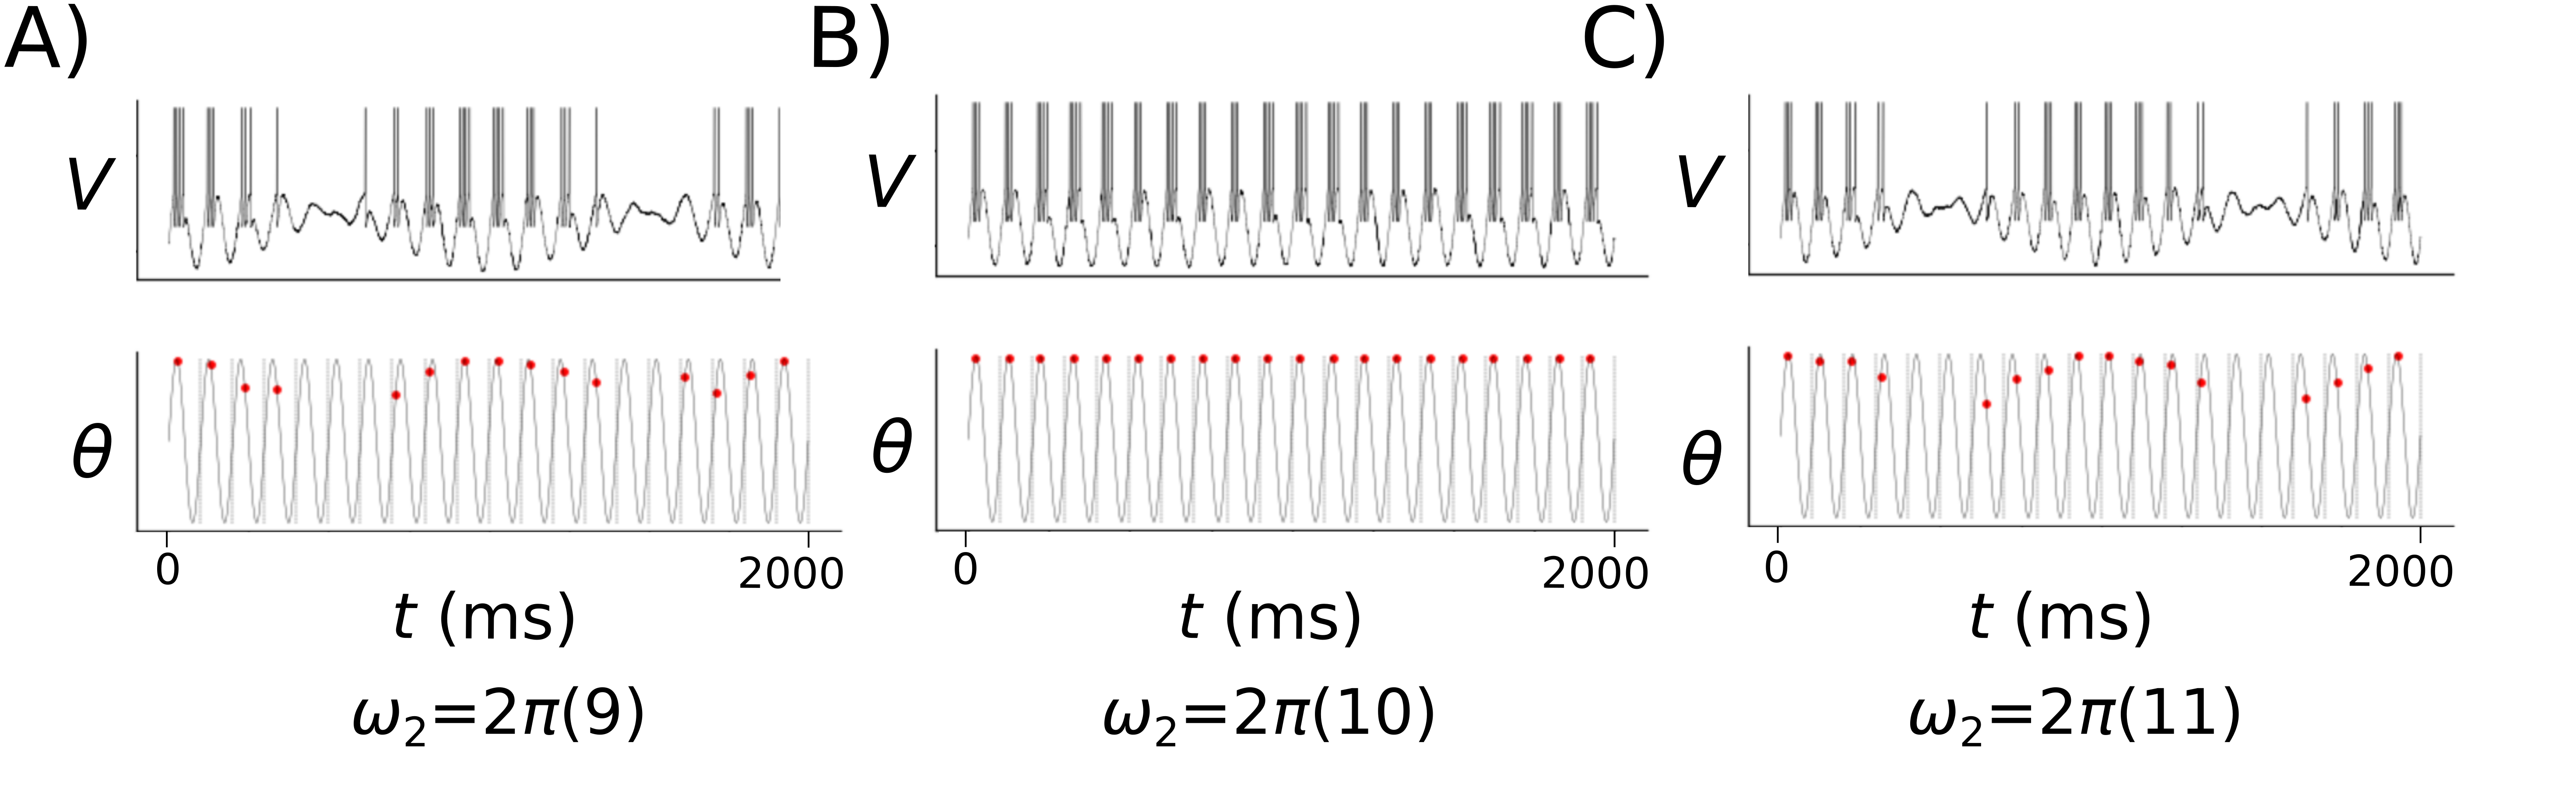
\includegraphics[width=200mm]{confirm_fig.png}}
  \end{center}
  {\bf Figure 1.} Two second time series generated by base model with varying
  interference frequency ($\omega_2$) plotted over a sinusoidal model of theta
  oscillation. Red dots superimposed on theta waveform indicate mean spike phase
  on each cycle. A) Interference frequency of 9 Hz results in model phase
  recession as per (2). B) Interference frequency of 10 Hz results in model phase
  locking as per (3). C) Interference frequency of 11 Hz results in model phase
  precession as per (4). While left unlabelled to reduce visual clutter, membrane
  potential remained above -120 mV over the 2 seconds plotted in A, B and C.

  \vspace{12pt}

  \begin{center}
    \makebox[\textwidth]{
\includegraphics[width=180mm]{base_model_RMQ.png}}
  \end{center}
  {\bf Figure 2.} Contour plots depicting RMQ return value ($\vartheta$) as a
  function of theta and interference oscillator amplitude for the base model
  under A) recession, B) locking and C) precession regimes. Contour plots are
  comprised of 1600 values of $\vartheta$ arranged in a 40x40 mesh according to
  the amplitudes of the dual oscillator input used to simulate the data from
  which it was derived. Magnitude and sign of $\vartheta$ is coded by colour
  according to the colourbar on the right.

  \vspace{12pt}

  \begin{center}
    \makebox[\textwidth]{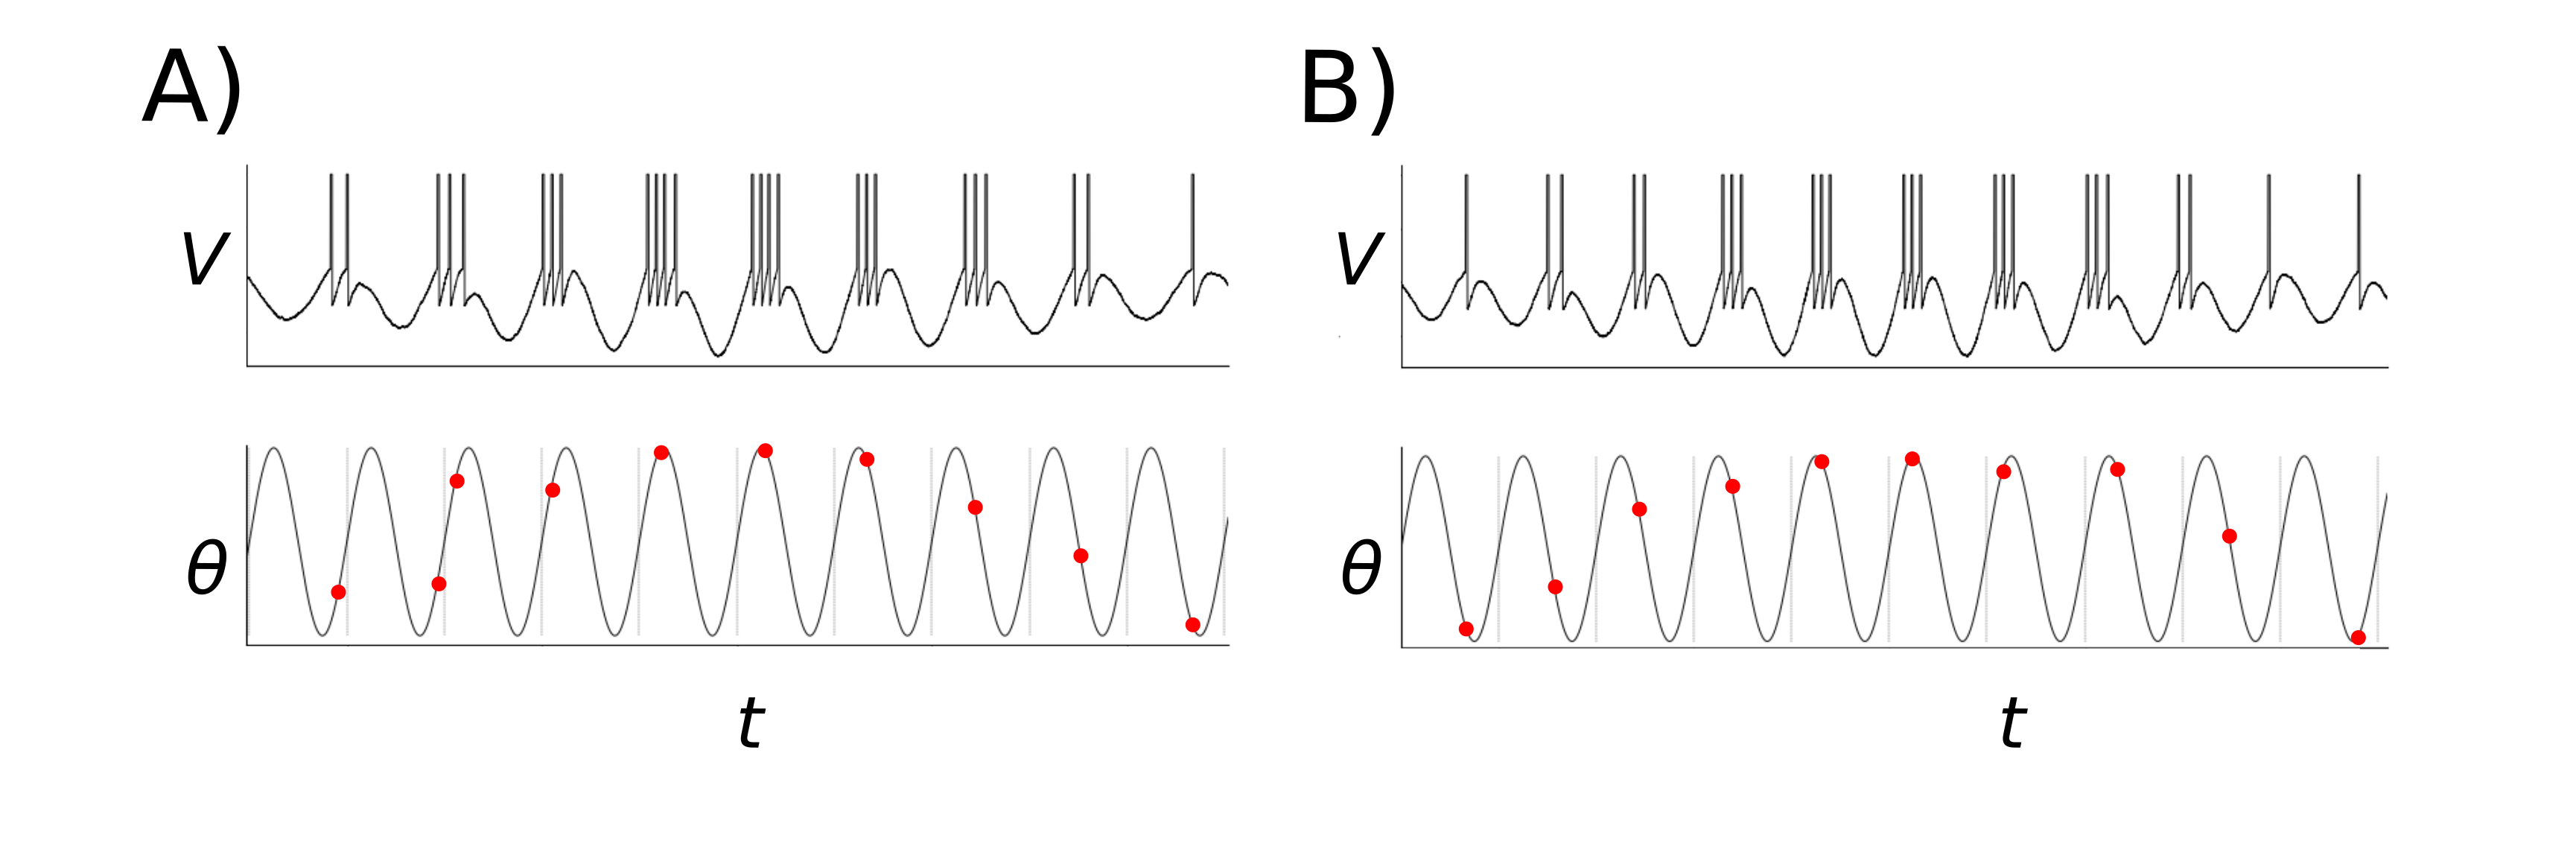
\includegraphics[width=200mm]{base_model_RMQ_zoom.png}}
  \end{center}
  {\bf Figure 3.} Sample time series generated by base model in regions where
  RMQ was erroneous. A) Data from precession region in figure 2.A for theta
  amplitude of 39 mV and interference amplitude of 50 mV. B) Data from
  locking region in figure 2.C where theta amplitude was 25 and interference
  amplitude was 43. Red dots superimposed on theta waveform indicate
  mean spike phase on each cycle.


  \begin{center}
    \makebox[\textwidth]{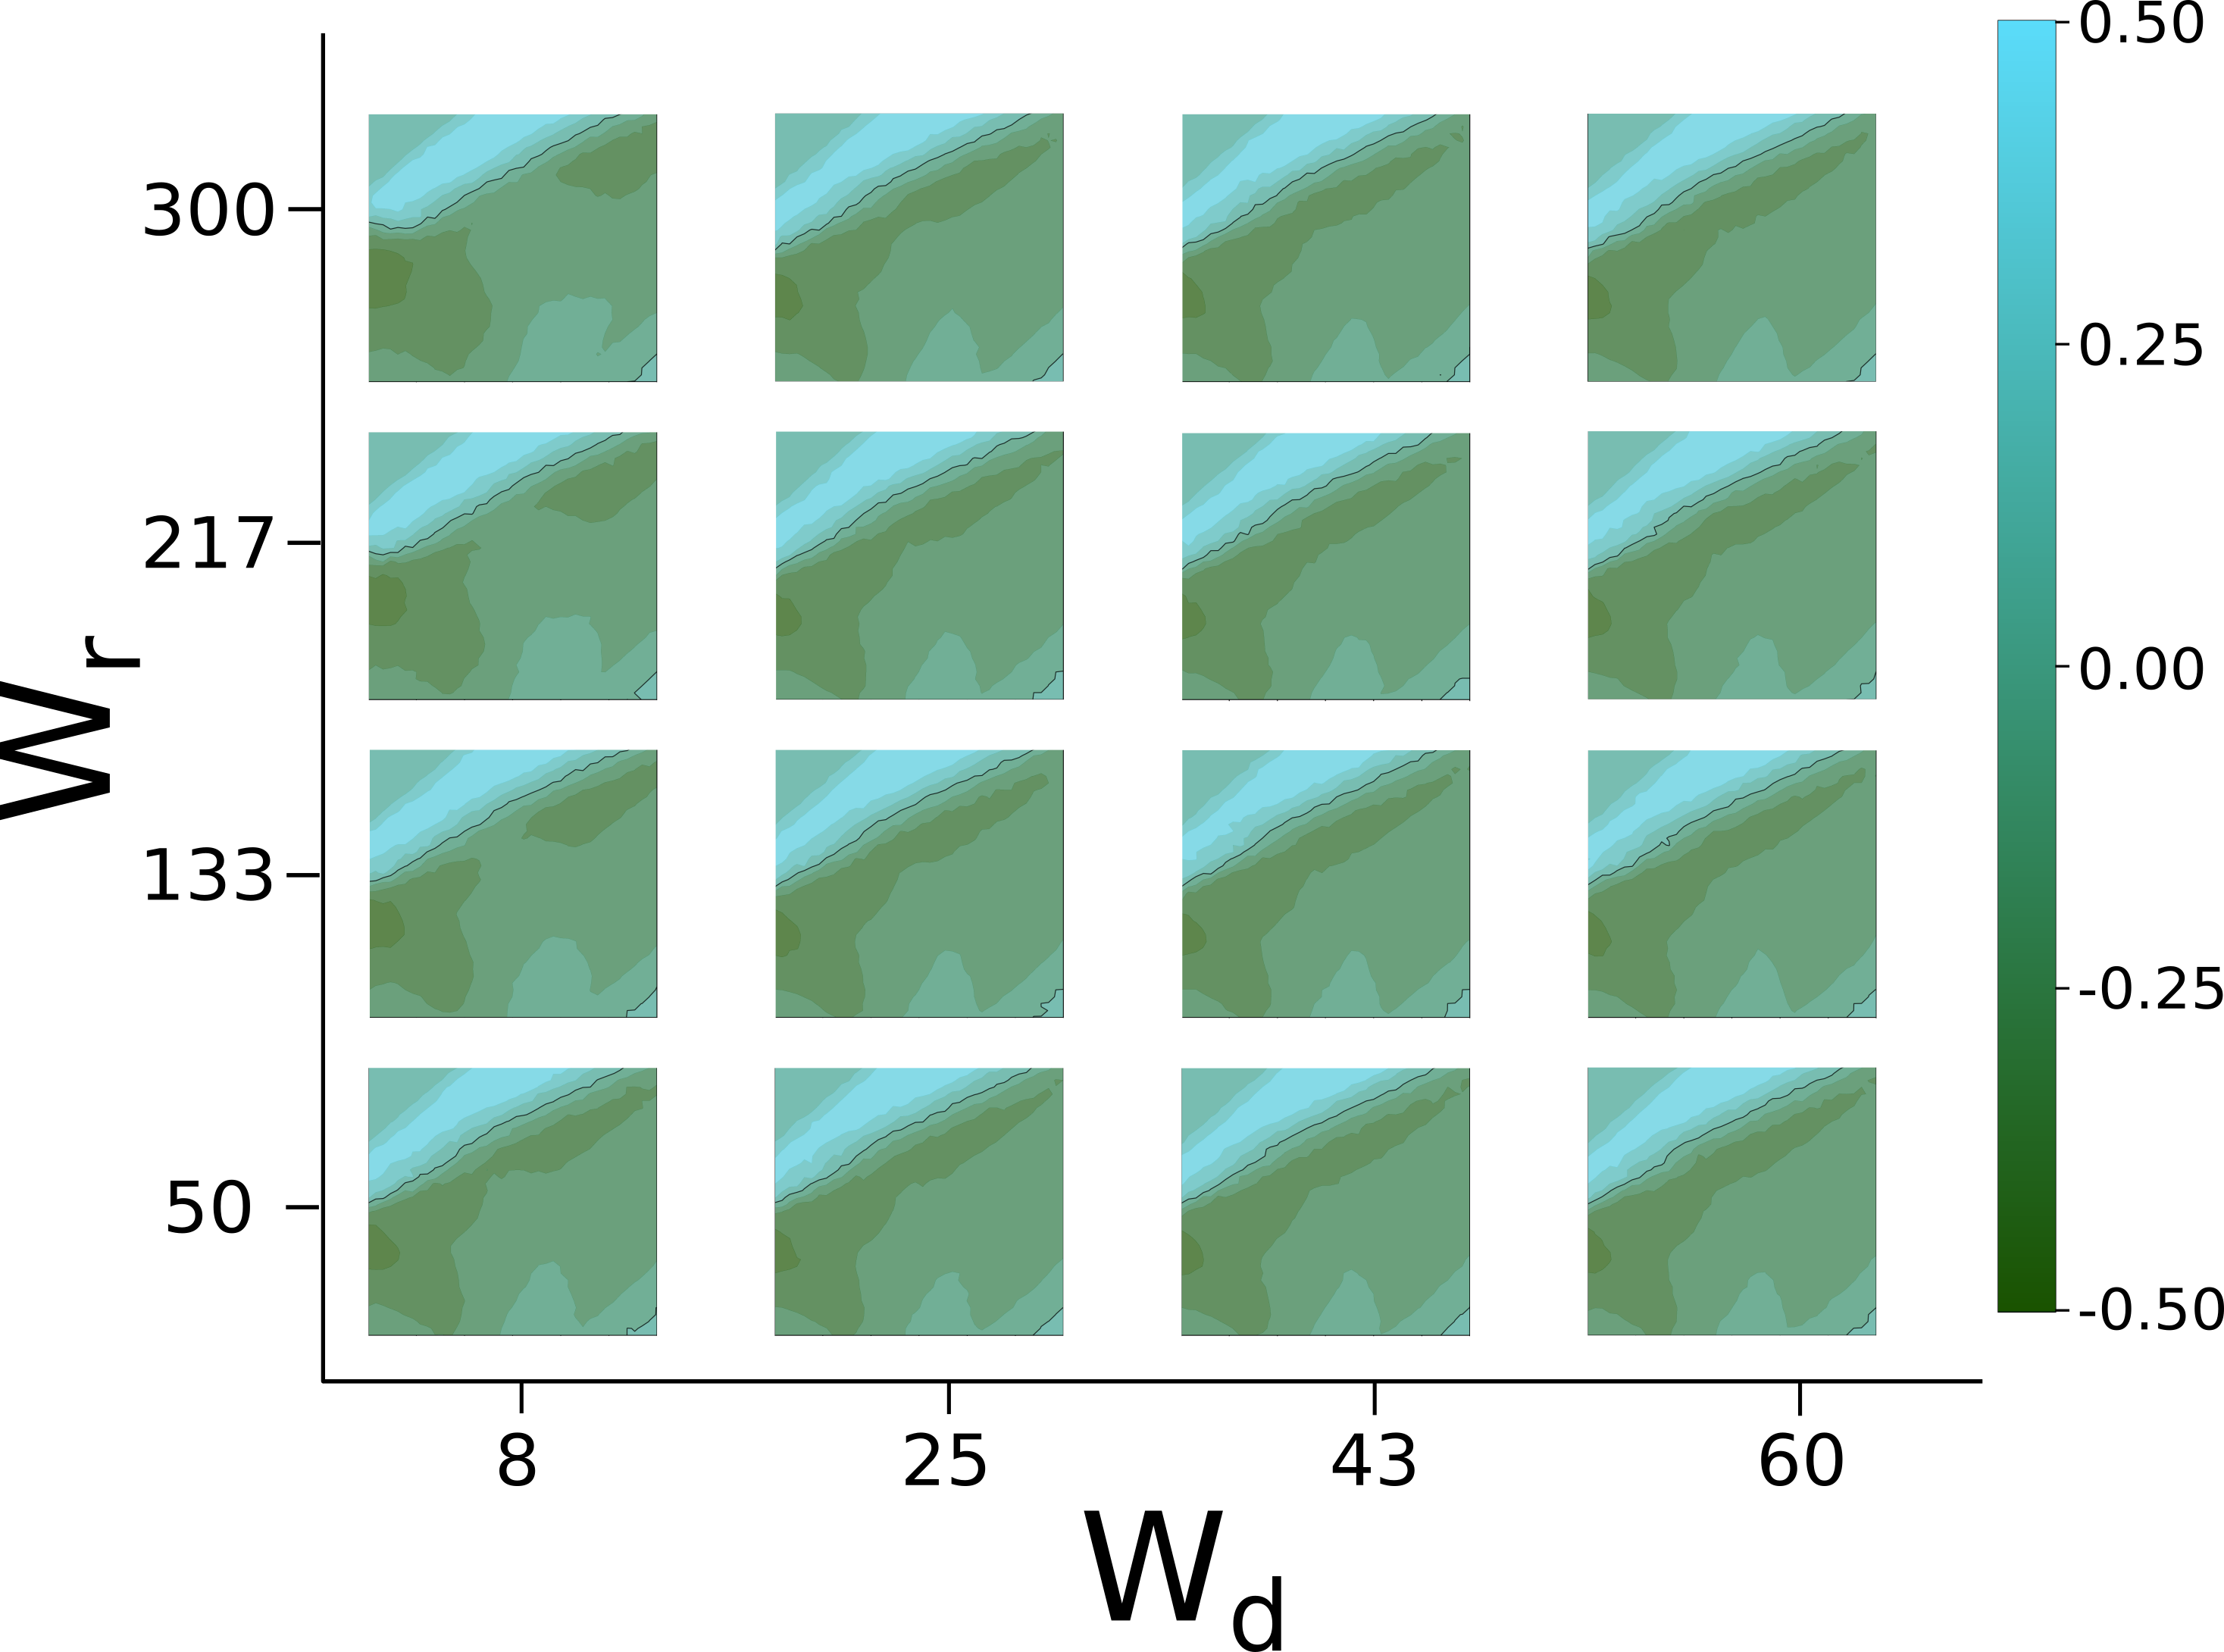
\includegraphics[width=110mm]{neurodyn_var_rec_RMQ.png}}
  \end{center}
  {\bf Figure 4.} Dual oscillator amplitude mesh contour plots depicting RMQ return value in
  the case of recession ground truth. Each plot is contructed in precisely the
  same way as those in figure 2, but with the exception that adaptation response
  ($W_r$) and decay ($W_d$) constants vary over the arranged grid. Magnitude and
  sign of $\vartheta$ is coded by colour according to the colourbar on the right.

  \vspace{12pt}

  \begin{center}
    \makebox[\textwidth]{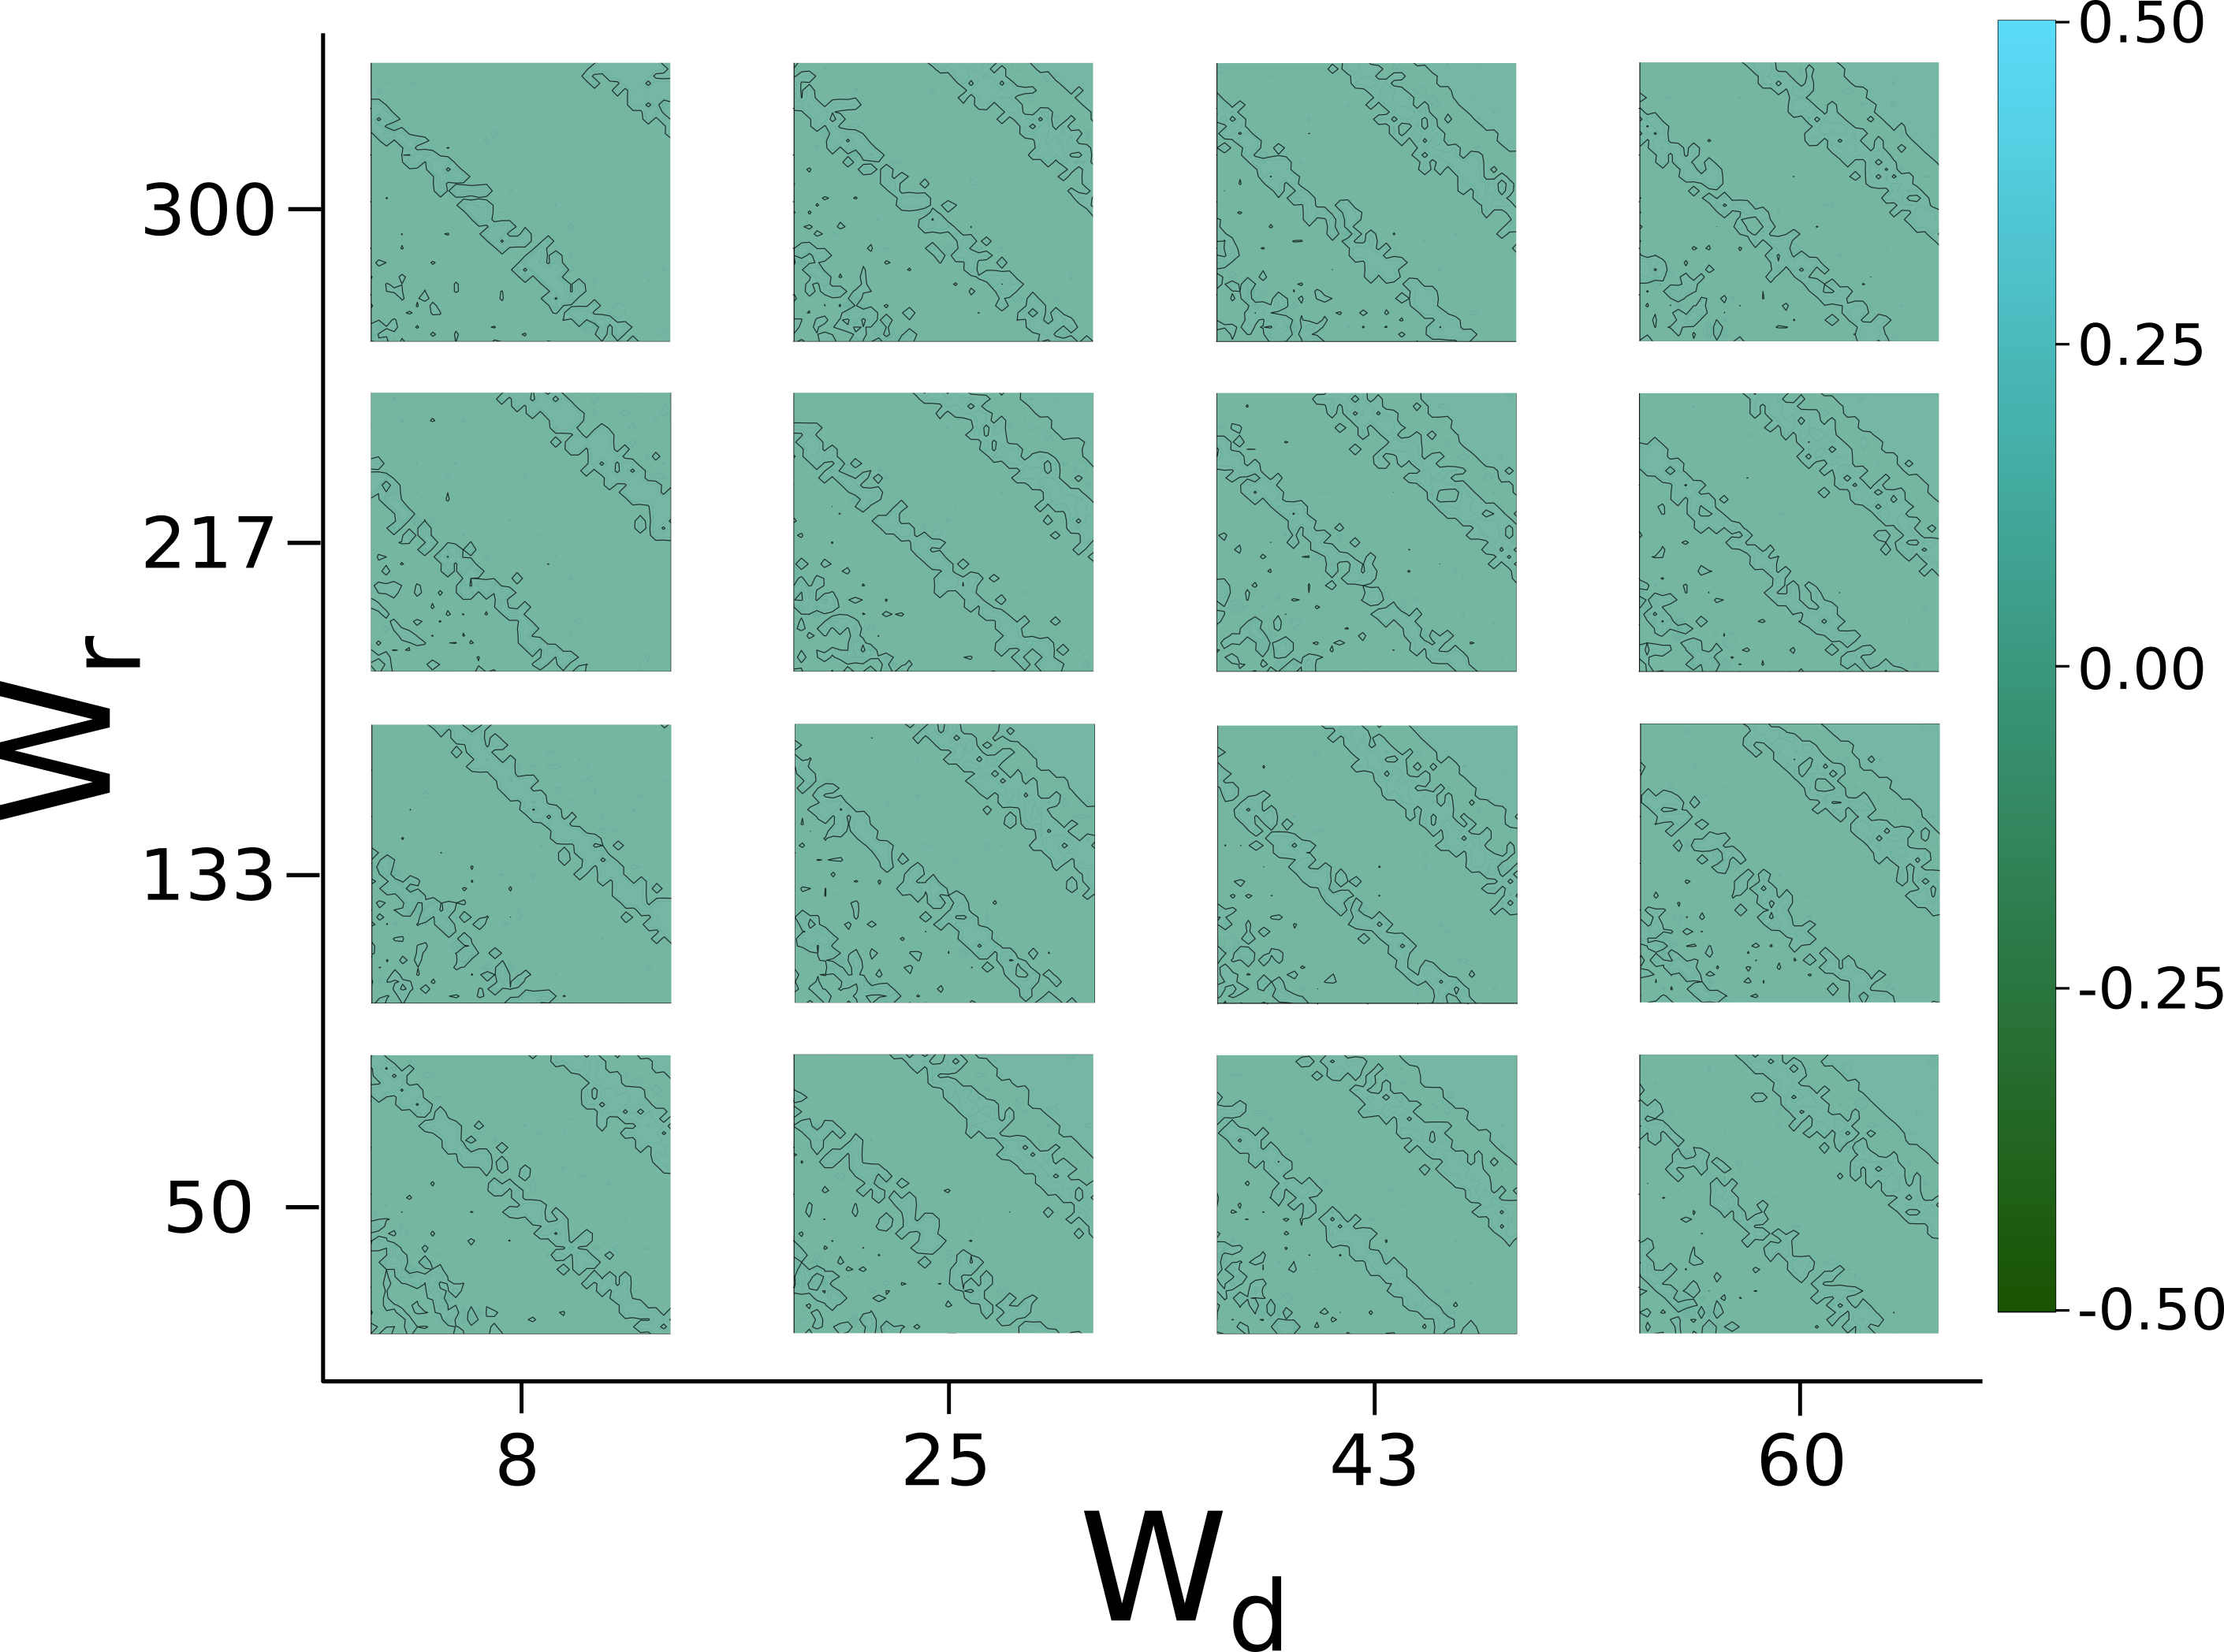
\includegraphics[width=110mm]{neurodyn_var_lock_RMQ.png}}
  \end{center}
  {\bf Figure 5.} Dual oscillator amplitude mesh contour plots depicting RMQ return value in
  the case of locking ground truth. Each plot is contructed in precisely the
  same way as those in figure 2, but with the exception that adaptation response
  ($W_r$) and decay ($W_d$) constants vary over the arranged grid. Magnitude and
  sign of $\vartheta$ is coded by colour according to the colourbar on the right.

  \vspace{12pt}

  \begin{center}
    \makebox[\textwidth]{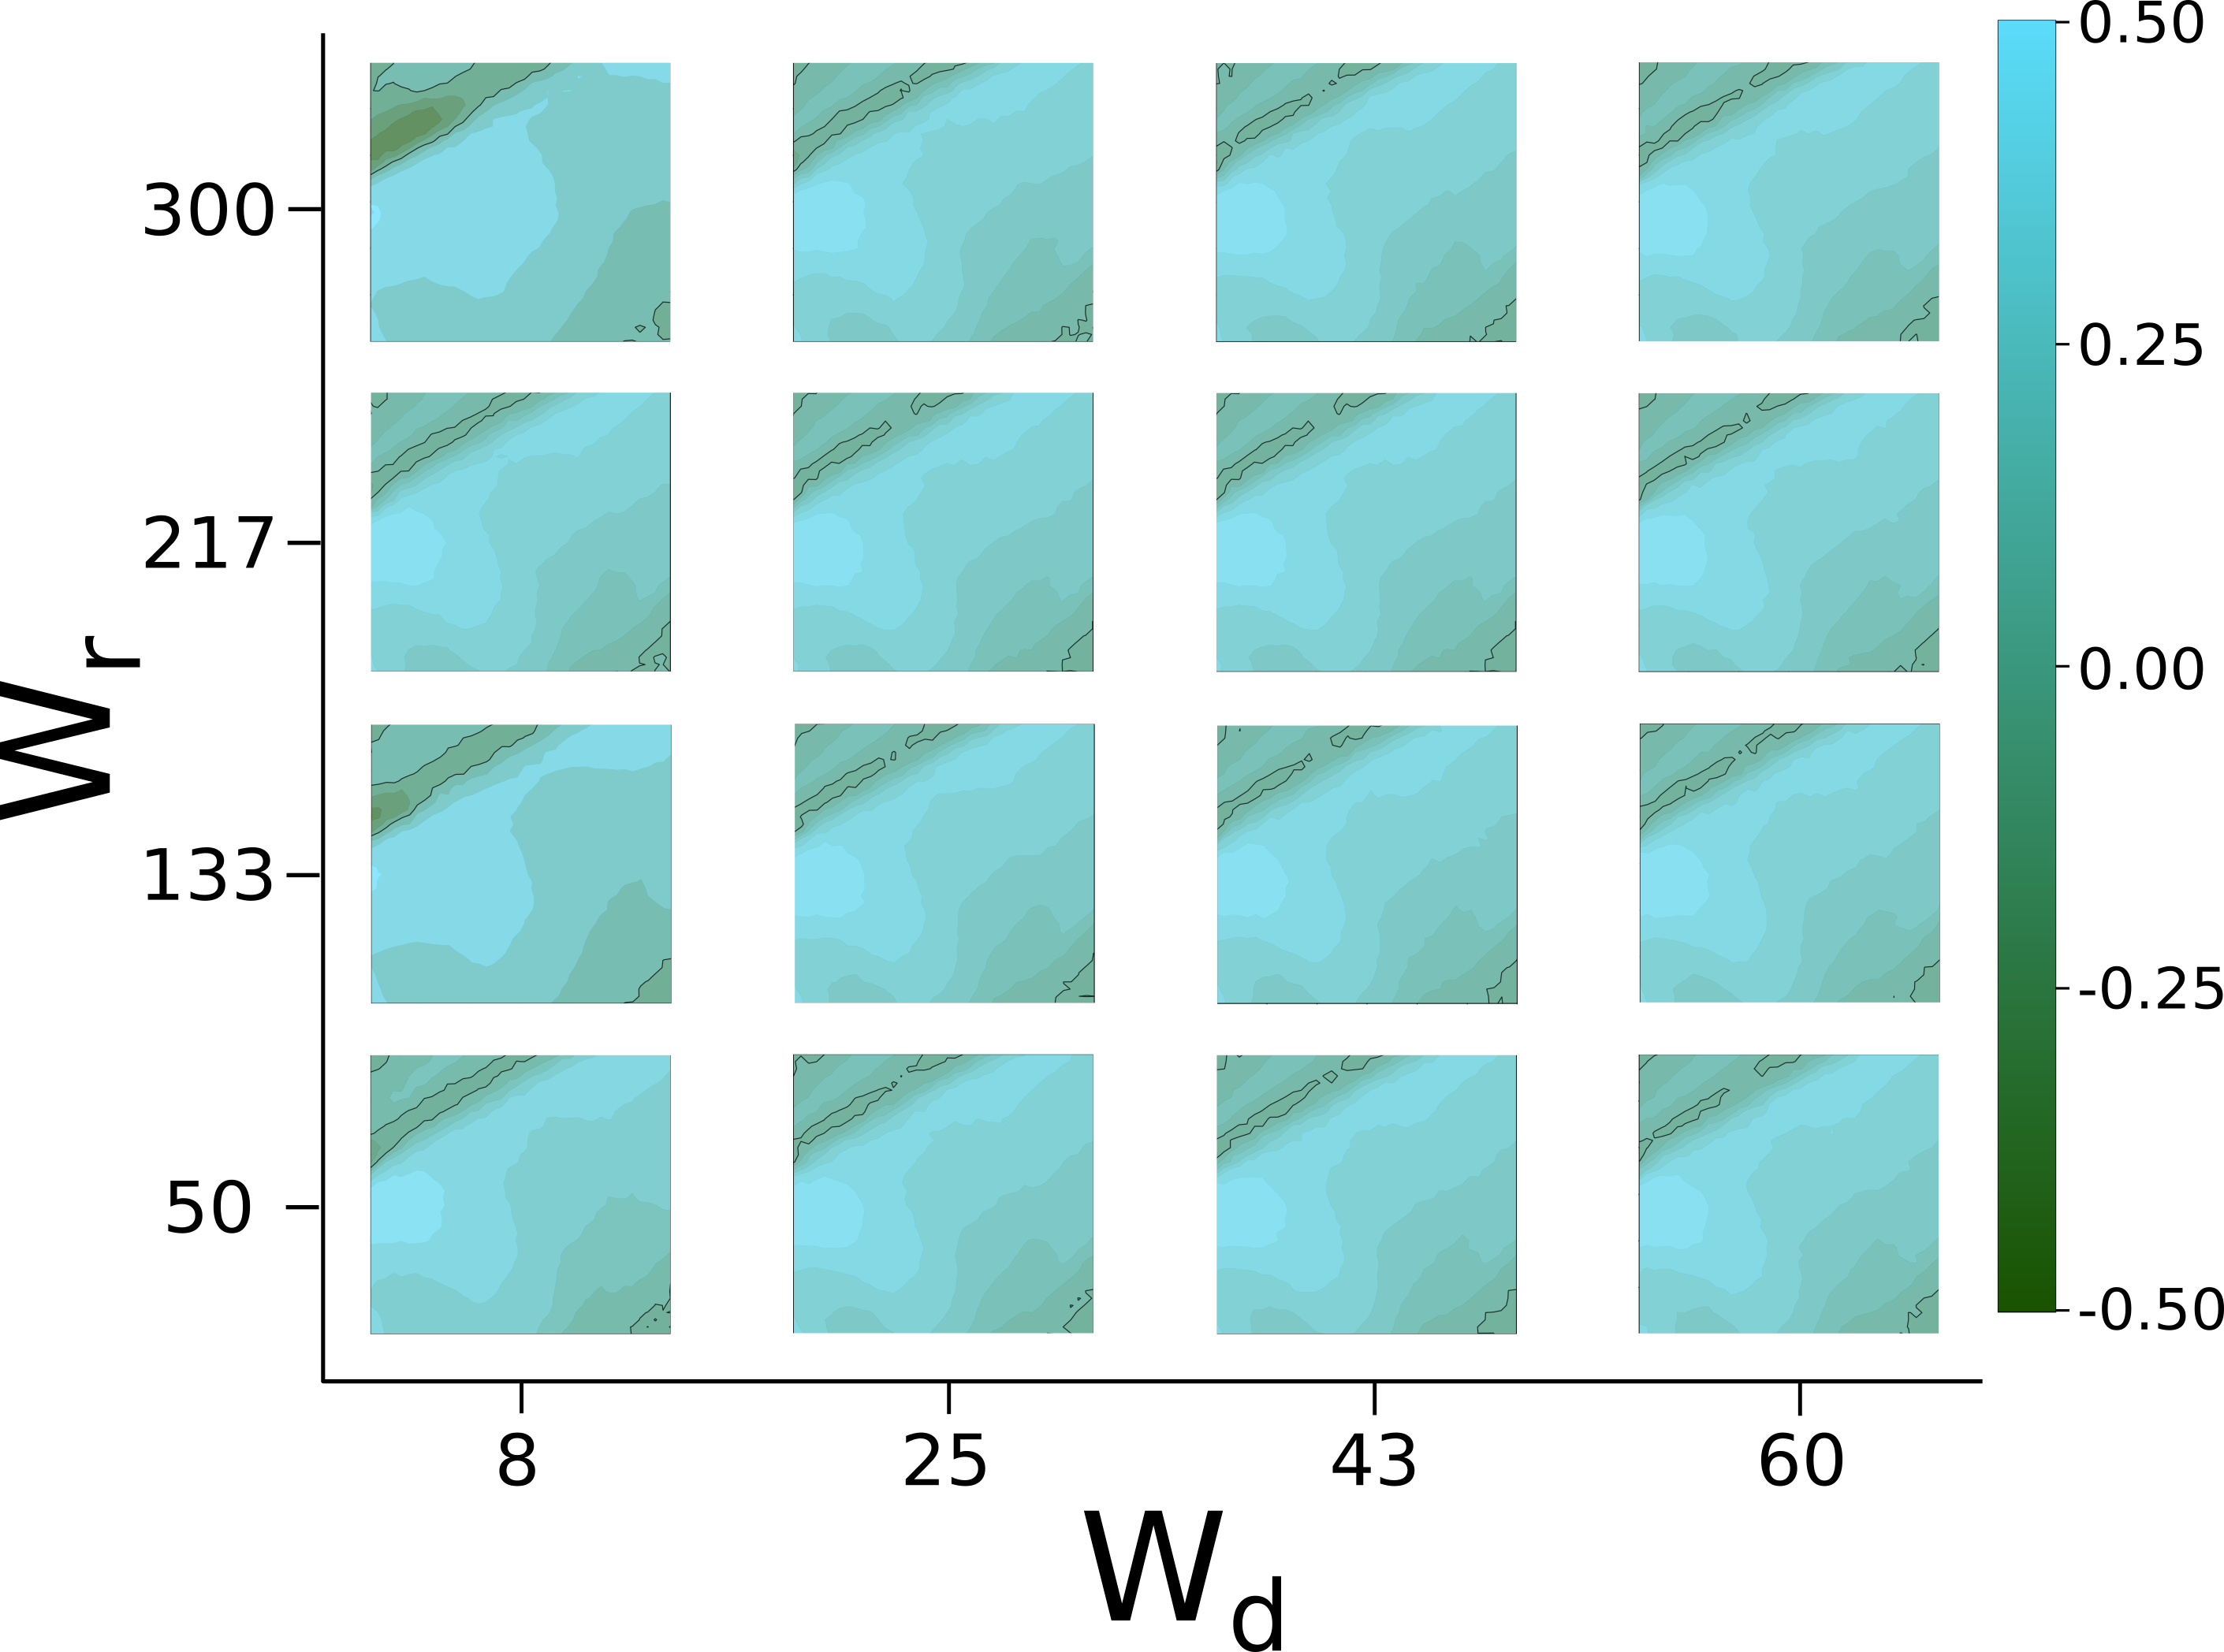
\includegraphics[width=110mm]{neurodyn_var_prec_RMQ.png}}
  \end{center}
  {\bf Figure 6.} Dual oscillator amplitude mesh contour plots depicting RMQ return value in
  the case of precession ground truth. Each plot is contructed in precisely the
  same way as those in figure 2, but with the exception that adaptation response
  ($W_r$) and decay ($W_d$) constants vary over the arranged grid. Magnitude and
  sign of $\vartheta$ is coded by colour according to the colourbar on the right.


\end{collapsable}

\end{document}
